\chapter[第五章]{} % (fold)
\label{cha:chapter5}

\section*{数值积分}

\subsection{问题}

\begin{equation}
    I = \int_0^1 \frac{\mathrm{arctan}x}{x^{\frac{3}{2}}} \mathrm{d}x
\end{equation}



\begin{enumerate}[(1)]
    \item 用 Romberg 公式计算改积分,使误差不超过 $\frac{1}{2}\times 10^{-7}$;
    \item ⽤复化 3 点 Gauss-Legendre 公式计算它,使误差不超过 $\frac{1}{2}\times 10^{-7}$。
\end{enumerate}

\subsection{分析}

\subsubsection{复化 Romberg 公式的分析}

\begin{enumerate}[(1)]
    \item 首先用递推关系求梯形公式:
    \begin{align}
        T_1 &= h(\frac{1}{2}f(a)+\frac{1}{2}f(b)) \\
        T_{2n} &= \frac{1}{2}T_n + \frac{h(n)}{2}\sum\nolimits_{n=0}^{n-1}f(x_{k+1/2})
    \end{align}

    \item 利用梯形公式求 Simpson 公式:
    \begin{equation}
        S_n(f) = \frac{4}{3}T_{2n}(f) - \frac{1}{3}T_n(f)
    \end{equation}

    \item 利用 Simpson 公式求 Cotes 公式:
    \begin{equation}
        C_n(f) = \frac{16}{15}S_{2n}(f)-\frac{1}{15}S_n(f)
    \end{equation}

    \item 最后用 Cotes 求 Romberg 公式:
    \begin{equation}
        R_n(f) = \frac{64}{63}C_{2n}(f)-\frac{1}{63}C_n(f)
    \end{equation}
\end{enumerate}

\subsubsection{Gauss-Legendre 求积公式分析}

\begin{enumerate}[(1)]
    \item $[-1,1]$ 上的3点Gauss-Legendre公式:
    \begin{equation}
        \int_{-1}^1 g(x)\mathrm{d}x \approx \frac{5}{9}g(-\sqrt{\frac{3}{5}}) + \frac{8}{9}g(0) + \frac{5}{9}g(\sqrt{\frac{3}{5}})
    \end{equation}

    \item 一般区间 $[a,b]$ 上的 Gauss 公式:
    
    令 $x_k = \frac{a+b}{2}+\frac{b-a}{2}t_k$,$A_k = \frac{b-a}{2}\tilde{A}_k$,$k=0:n$

    \item 由于 Gauss 求积公式的节点不具有递推性,因此用截断误差计算节点的数量, Gauss-Lengdre 公式的截断误差为:
    \begin{multline}
        R(f) = \int _a^b f(x)\mathrm{d}x - \sum\nolimits_{k=0}^n A_kf(x_k) = \frac{f^{2n+2}(\xi)}{(2n+2)!} \int_a^b W_{n+1}^2(x)\mathrm{d}x, \\
        W_{n+1}(x) = \prod\nolimits_{j=0}^n (x-x_j), \quad \xi \in (a,b)
    \end{multline}

\end{enumerate}

\subsubsection{待积函数分析}

待求积分的函数为:

\begin{equation}
    g(x) = \frac{\mathrm{arctan}x}{x^{3/2}}
\end{equation}

该函数的图像如图\ref{fig:f}所示,是一个奇异函数,在 $x=0$ 处有奇异点,值为 $+\infty$,用 Romberg 公式求积时需要用到 $x=0$ 处的值。在 $[0,x_0]$ 上的积分用右矩形公式的两倍近似,即 $\int_0^{x_0} g(x) \mathrm{d}x \approx 2\cdot x_0 \cdot g(x_0) $,保证近似值小于一半的误差限,即 $2\cdot x_0 \cdot g(x_0) \leq 1/2 \times 1/2 \times 10^{-7}$;

为了减少计算量,在 $[x_0, 1]$ 上,做分段积分,分别对 $[x_0,1\times 10^{-9}]$、$[1\times 10^{-9},1\times 10^{-4}]$、$[1\times 10^{-4},1]$做Romberg积分,每一段的误差都要求小于 $1/6 \times 1/2 \times 10^{-7}$,这样保证总的误差不超过 $ 1/2 \times 10^{-7}$。

\begin{figure}[ht]
    \centering
      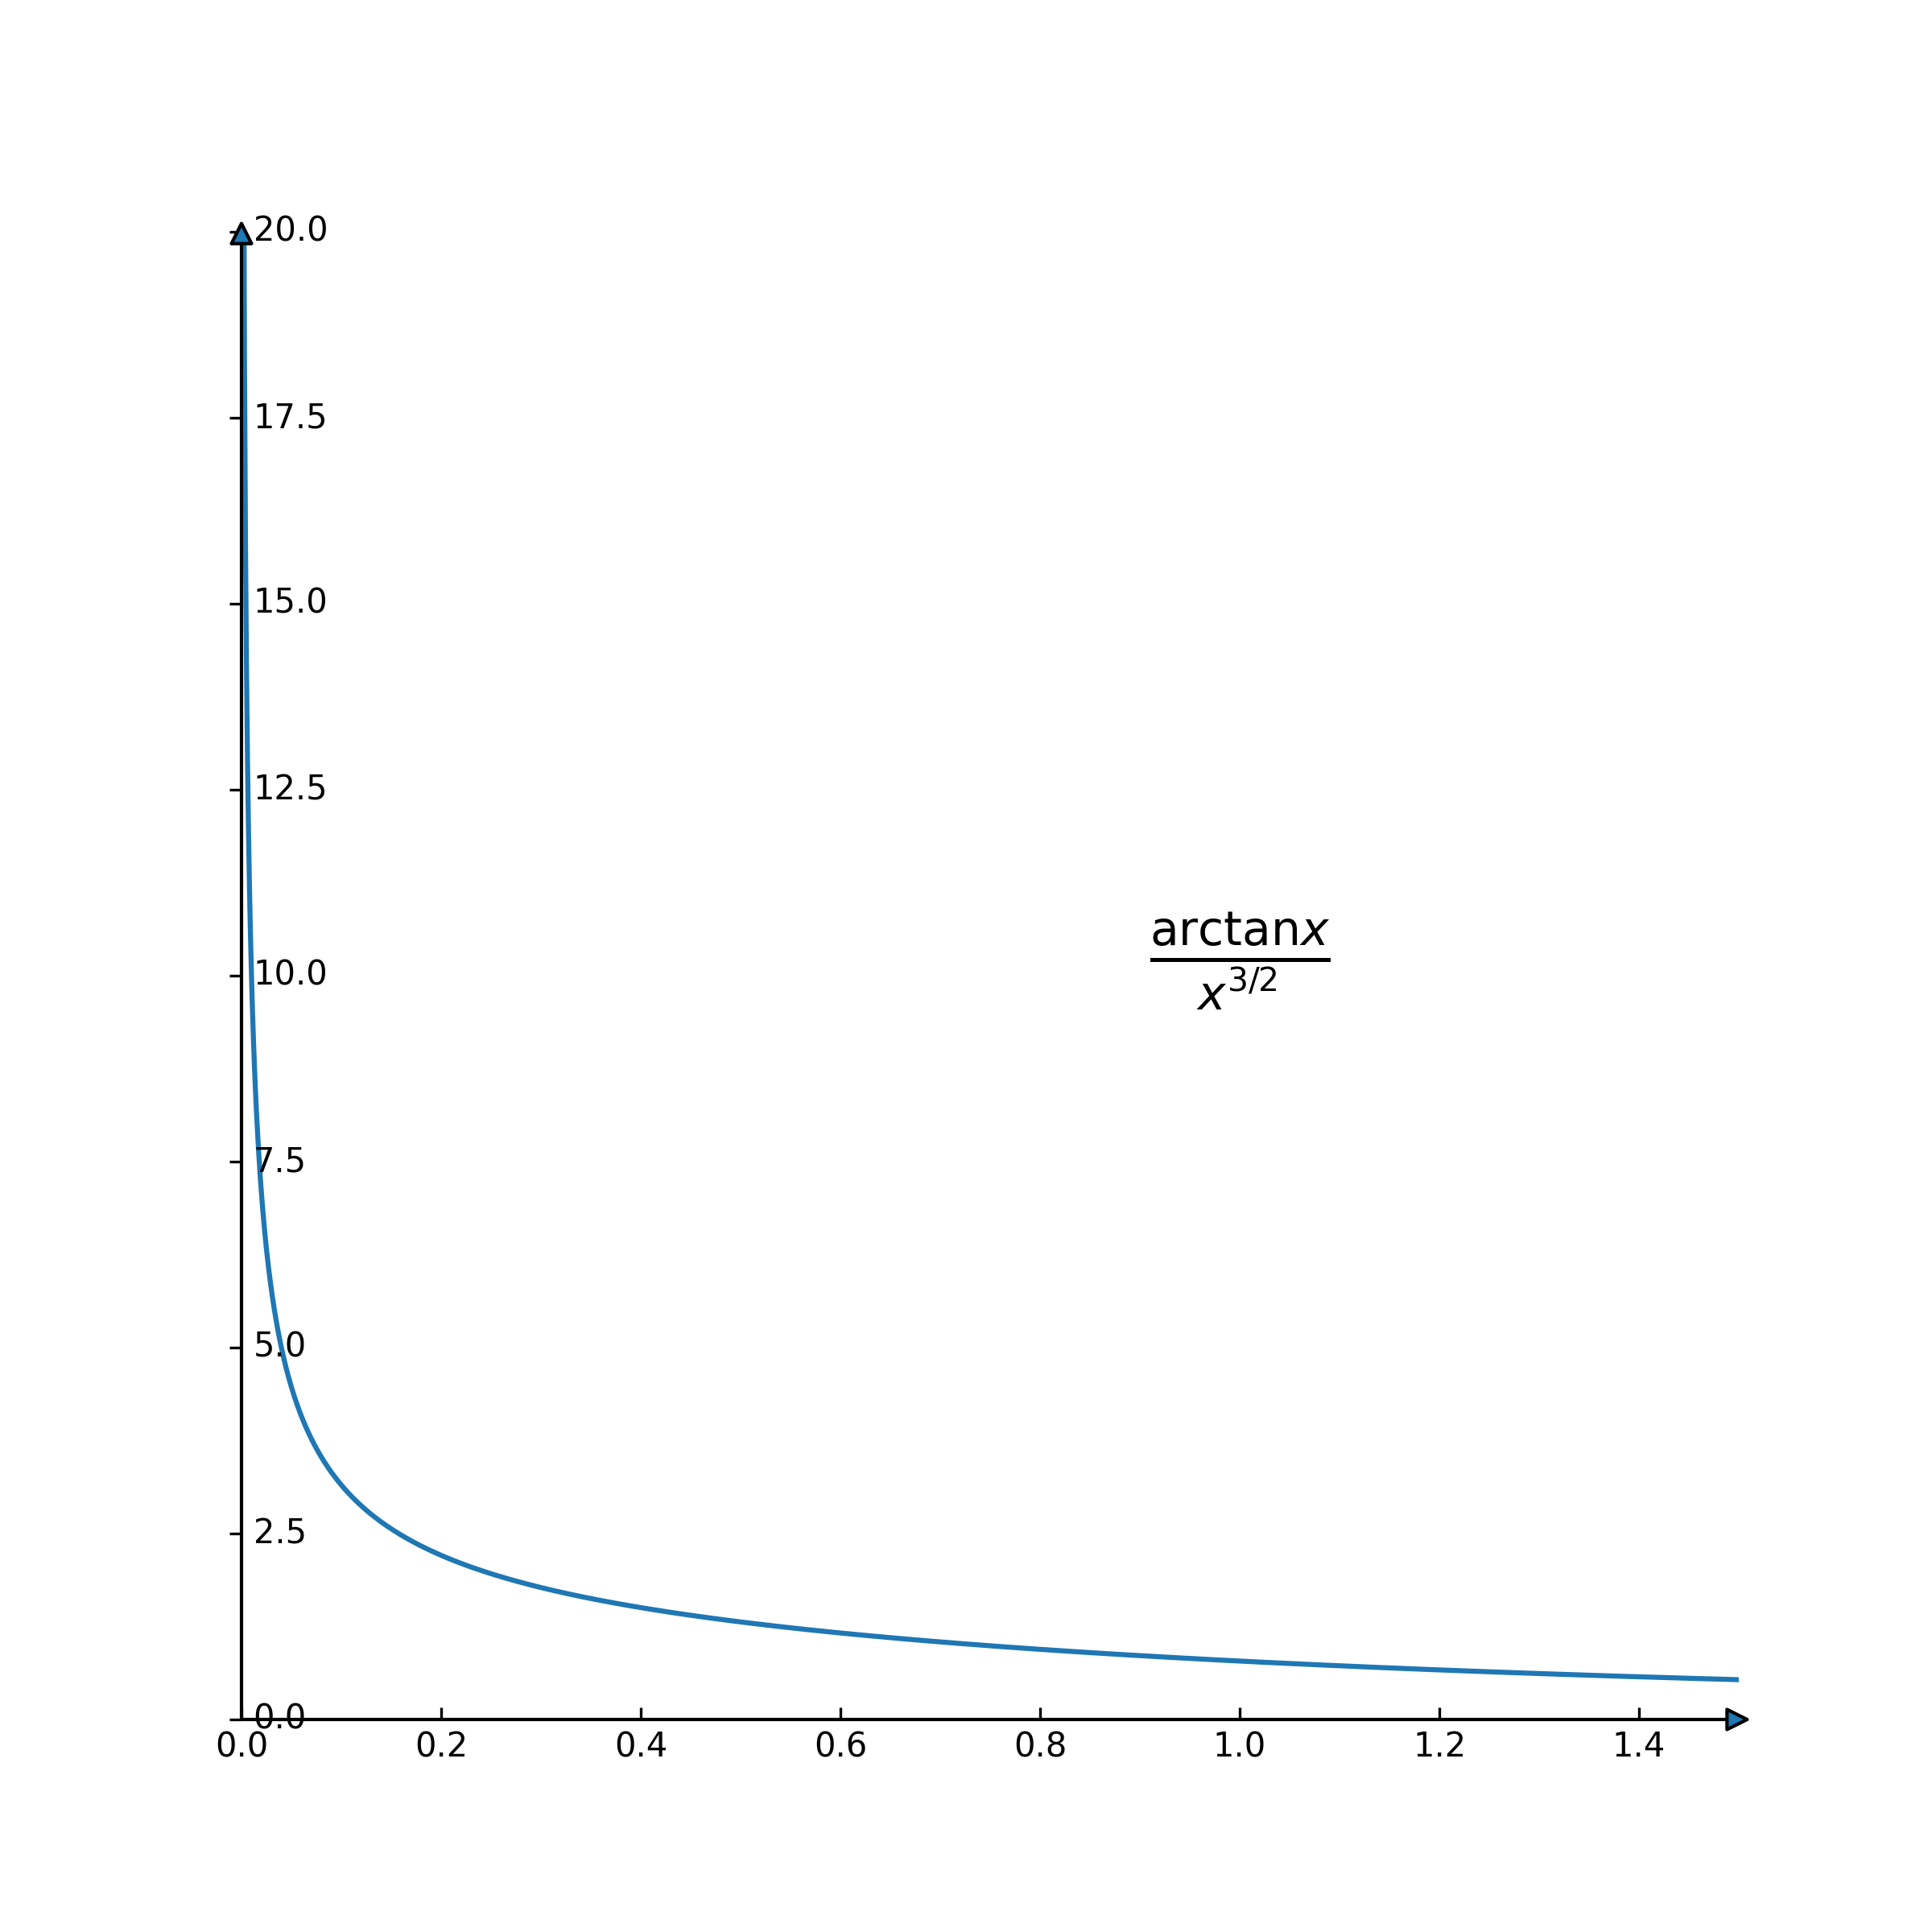
\includegraphics[width=0.5\textwidth]{fq3}
      \caption{$(\mathrm{arctan}x)/(x^{3/2})$ 图像}
      \label{fig:f}
\end{figure}

\subsection{程序}

\begin{lstlisting}[style = python]

\end{lstlisting}

\subsection{算例}

\begin{equation}
    I = \int_0^1 \frac{\mathrm{arctan}x}{x^{\frac{3}{2}}} \mathrm{d}x
\end{equation}

用 Romberg 求积公式的实际积分区间是$[1.110223025\times 10^{-16},1\times 10^{-9}]$、$[1\times 10^{-9},1\times 10^{-4}]$、$[1\times 10^{-4},1]$,计算出来的结果是:$1.897097415$;

用 Gauss-Legendre 求积公式计算出来的结果是:$??$。

\subsection{结论}

算术解的结果为:
\begin{multline}
    y = -\frac{log(x - \sqrt{2x} + 1)}{\sqrt{2}} + \frac{log(x + \sqrt{2x} + 1)}{\sqrt{2}} {} \\
    - \sqrt{2} tan^{-1}(1 - \sqrt{2x}) + \sqrt{2} tan^{-1}(\sqrt{2x} + 1) - \frac{2 tan^{-1}(x)}{\sqrt{x}}
\end{multline}

因此准确解是:$1.897095623$。

\subsubsection{复化 Romberg 公式}

对比准确解可以看到,实际误差为$1.8\times 10^{-6}$,大于所要求的的 $\frac{1}{2}\times 10^{-7}$,且计算值略大于真实值,分析后应该是在 $[x_0,1\times 10^{-9}]$ 这段上误差太大,因为在 $x_0$ 处的值还是太大了,因此将这段的误差设为 $1/2\times 10^{-9}$,其他两段的误差设定保持 $1/6 \times 1/2 \times 10^{-7}$,再次计算出来的结果是 $1.897095976$,误差是 $3.5\times 10^{-7}$,达到了误差的要求。

在没有分段积分时,程序跑了一周多也没有收敛到误差要求内,在设定好合适的分段积分区间后,程序只运行了 0.2 s 就收敛到误差要求内,效率提升很大。

\subsubsection{Gauss-Legendre 求积公式}



% chapter chapter5 (end)